%%%%%%%%%%%%%%%%%%%%%%%%%%%%%%%%%%%%%%%%%%%%%%%%%%%%%%%%%%%%%%%%%%%%%%%%%%%%%%%%%
% MICAI / Springer LNCS submission -- REDUCED (conference-length) version
% Trimmed from the full 20pp manuscript; the full version is main.tex.
% MICAI / Springer LNCS submission
% "Feasibility-Preserving Multi-Objective Harris Hawks Optimization
%  for Employment-Based Visa Allocation"
%
% Compile: pdflatex main  (x2-3 passes to resolve refs)
% Bibliography: inline thebibliography (no BibTeX pass needed).
%
% ---------------------------------------------------------------------------
% DOUBLE-BLIND SUBMISSION:  MICAI reviews anonymously. To anonymize, (1) comment
% out the \author / \institute blocks below and use the ANONYMOUS block marked
% "% >>> REVIEW", (2) comment out the Acknowledgements, and (3) remove the repo
% URL in the Data Availability statement. The body is otherwise identical.
%%%%%%%%%%%%%%%%%%%%%%%%%%%%%%%%%%%%%%%%%%%%%%%%%%%%%%%%%%%%%%%%%%%%%%%%%%%%%%%%%
\documentclass[runningheads]{llncs}

% --- A4 trap fix: force a true A4 MediaBox without touching the LNCS text block.
\AtBeginDocument{\pdfpagewidth=210mm \pdfpageheight=297mm}

\usepackage[T1]{fontenc}
\usepackage[utf8]{inputenc}
\usepackage{lmodern}   % scalable fonts (required for microtype expansion)
\usepackage{graphicx}
\usepackage{xcolor}
% amsmath + llncs emit one benign "Unable to redefine math accent \vec" warning
% (modern robust accents); silence just that during amsmath's load, then restore.
\makeatletter
\let\vp@oldwarn\PackageWarningNoLine
\renewcommand\PackageWarningNoLine[2]{}
\usepackage{amsmath,amssymb}
\let\PackageWarningNoLine\vp@oldwarn
\makeatother
\setlength{\emergencystretch}{1em}  % gentle: absorb tight lines in narrow columns
\usepackage{booktabs}
\usepackage{array}
\usepackage{float}
\usepackage{algpseudocode}
% lightweight "algorithm" float (avoids the algorithms bundle; on Overleaf the
% standard \usepackage{algorithm} also works and yields the same result)
\floatstyle{ruled}
\newfloat{algorithm}{tbp}{loa}
\floatname{algorithm}{Algorithm}
\usepackage{microtype}
\usepackage[hidelinks]{hyperref}
\usepackage{url}
\renewcommand\UrlFont{\color{black}\rmfamily}

% consistent metric/acronym capitalization
\newcommand{\HV}{\textsf{HV}}
\newcommand{\IGD}{\textsf{IGD}}

\graphicspath{{figures/}}

\begin{document}

\title{A Two-Condition Diagnostic for Decoder-Based\texorpdfstring{\\}{ }Multi-Objective Search: When Blind Sampling\texorpdfstring{\\}{ }Beats a Mismatched NSGA-II}
\titlerunning{Two-Condition Diagnostic for Decoder-Based Search}

% >>> CAMERA-READY (named) author block:
\author{Javier Augusto Rebull Saucedo\orcidID{0009-0008-2089-5274} \and
Yazmin Ivonne Flores Martinez\orcidID{0009-0002-6848-1608} \and
Ra\'ul Gibran Porras Alaniz\orcidID{0000-0002-6772-5351}}
\authorrunning{J.\,A. Rebull Saucedo et al.}
\institute{Maestr\'ia en Inteligencia Artificial y Anal\'itica de Datos, Universidad Aut\'onoma de Ciudad Ju\'arez, Ciudad Ju\'arez, Chihuahua, M\'exico\\
\email{rebull@outlook.com}}

% >>> REVIEW (anonymous) author block -- swap in for double-blind submission:
% \author{Anonymous Author(s)}
% \authorrunning{Anonymous}
% \institute{Institution withheld for review}

\maketitle

\begin{abstract}
Many hard-constrained combinatorial problems are solved by pairing a metaheuristic with a feasibility-preserving decoder, yet the true driver of performance is seldom isolated. We isolate it on a calibrated case study: allocating 140{,}000 U.S.\ employment-based visas per year under a per-country ceiling and spillover cascade---a three-objective integer program with six hard constraints. Multi-objective Harris Hawks Optimization (MOHHO) searches it through a smallest-position-value random-key mapping and a greedy assignment feasible by construction---no penalties, no repair. A controlled nine-method ladder shows why search fails. Blind random sampling beats a standard real-coded NSGA-II and a naive swarm because their realized search is \emph{degenerate}: interpolating operators barely change the decoded order, or gated acceptance freezes the population. The two corresponding conditions are necessary there, not sufficient. A BRKGA-style biased-uniform crossover that does change the order under diversity-preserving selection only ties blind sampling, and a registered eleven-level disruption sweep finds hypervolume nearly flat within that family---only the right kind of order renewal (a competent random-key swarm or permutation-native operators) reaches the top tier. We package these measurements as a cheap a priori screening diagnostic and stress it with registered prospective tests: the two-condition core predicted correctly; the landscape label and dose--response reading did not. Across knapsack, traveling-salesman, flow-shop, and set-covering replications, the best ladder method satisfies both conditions, while the mismatched genetic algorithm's collapse below blind sampling is landscape- and configuration-specific. A Taguchi design fixes the shared parameters; the recovered front Pareto-dominates the first-in, first-out incumbent and yields an auditable trade-off menu.

\keywords{Multi-objective optimization \and Harris Hawks Optimization \and Constraint handling \and Random-key decoder \and Permutation encoding \and Taguchi design of experiments \and Resource allocation}
\end{abstract}

%===============================================================================
\section{Introduction}
\label{sec:intro}

Each fiscal year the United States Congress authorizes approximately 140{,}000 employment-based (EB) immigrant visas, distributed across five categories (EB-1 to EB-5). Two structural rules govern the distribution: a \emph{per-country ceiling} ($P_c \approx 25{,}620$ visas, the statutory 7\,\% cross-preference limit over the combined family-sponsored and employment-based preference totals~\cite{uscis}) that no single country may exceed, and a \emph{spillover} mechanism that cascades unused visas across categories (EB-4/5 $\rightarrow$ EB-1 $\rightarrow$ EB-2 $\rightarrow$ EB-3). The incumbent system processes petitions strictly first-in, first-out (FIFO) by priority date. In our calibrated instance these rules create measurable inefficiencies: two countries concentrate roughly three-quarters of demand (India $\approx 63\,\%$, China $\approx 14\,\%$) with 10--13-year waits, while the ceiling clash leaves thousands of visas unused.

This matters beyond accounting. Behind every backlogged petition is a household whose relocation and reunification hinge on a priority date. The problem admits three legitimate, mutually conflicting goals: serve the longest-waiting petitions (\emph{efficiency}), distribute opportunity evenly across nationalities (\emph{equity}), and waste no visas (\emph{utilization}). No single allocation optimizes all three; the decision-relevant object is the set of best compromises---a Pareto front. Algorithmic assignment of people to scarce slots has been studied for refugee resettlement~\cite{bansak}; our contribution is methodological, not a new matching design.

Computing that front is hard for three reasons. First, the allocation is \emph{combinatorial}: it assigns integer visa counts to 105 country$\times$category groups under six simultaneous constraints, and its feasible set generalizes the multidimensional knapsack problem, which is NP-hard~\cite{garey}. Second, the objectives are genuinely conflicting, so the solution is a front rather than a point. Third, the \emph{hard constraints} are unforgiving: a continuous metaheuristic naturally proposes infeasible candidates, and penalties or aggressive repair either require delicate tuning or distort the search landscape.

We address these challenges with a multi-objective adaptation of Harris Hawks Optimization (MOHHO) whose centerpiece is a \emph{feasibility-preserving decoder}. Our central contribution is methodological: a controlled, mechanistically explained account---developed on the visa problem and stress-tested across four structurally distinct multi-objective problems---of when decoder-based search beats blind sampling, distilled into a two-condition diagnostic that a practitioner can run before committing a full experimental budget. Concretely, this paper makes five contributions. \emph{(i)}~A decoder that couples a smallest-position-value (SPV) random-key mapping with a deterministic greedy assignment, guaranteeing all six hard constraints \emph{by construction}---without penalties or repair, and therefore without perturbing the search landscape. \emph{(ii)}~A calibrated, constraint-heavy allocation case study on which a multi-objective Harris Hawks optimizer with a crowding-pruned external archive recovers a Pareto front of policy trade-offs that dominates the FIFO incumbent. \emph{(iii)}~A Taguchi L9 design that fixes the population size and iteration budget shared by every ladder method, so that cross-method comparisons are not confounded by per-method tuning. \emph{(iv)}~A controlled nine-method ladder (with \emph{Discrete-MOHHO} as the swarm-side mechanism check), a $2\times2$ isolation experiment, and a direct operator-order-preservation measurement (Kendall $\tau$ through the decoder); together these yield the two-condition diagnostic---operators must change the decoded order and selection must preserve diversity---validated predictively on a BRKGA-style crossover not used to formulate it, which sharpens the two conditions from a binary rule to a necessary-but-graded one. \emph{(v)}~A reproducible empirical protocol (30 seeds, omnibus Friedman/Nemenyi tests with effect sizes, FIFO domination, five perturbed-demand instances) and a four-structure generalization (the visa plus knapsack, traveling salesman, flow-shop) plus a registered prospective test on a fifth (set covering), separating what transfers---the best ladder method on every structure satisfies both conditions, the family second-order among them---from what is landscape- and configuration-specific (the collapse of a genetic algorithm (GA) below random sampling).

%===============================================================================
\section{Background and Related Work}
\label{sec:related}

Harris Hawks Optimization (HHO)~\cite{heidari} is a population-based metaheuristic whose prey \emph{escape energy} $E$ drives a continuous exploration--exploitation transition, with optional L\'evy-flight dives. It has been extended to multiple objectives via external archives, elitist non-dominated sorting, and grid indices~\cite{choo,jangir,cerci,kusoglu}; these variants are validated mostly on continuous benchmarks, leaving their use on constrained combinatorial allocation---where feasibility, not convergence, is the binding difficulty---comparatively unexplored.

We bridge continuous search and combinatorial structure with random keys~\cite{bean}: a real vector is decoded to a feasible permutation by sorting (the smallest-position-value, SPV, rule~\cite{tasgetiren}). How much an operator step changes the decoded phenotype is the classical representation-\emph{locality} question, formalized by Rothlauf~\cite{rothlauf} and measured for decoder-based evolutionary algorithms by Raidl and Gottlieb~\cite{raidl}---the lens our Kendall-$\tau$ measurement instantiates (their \emph{heuristic-bias} half makes blind sampling through a greedy decoder a semi-greedy multistart in the GRASP (greedy randomized adaptive search procedure) sense~\cite{feo}). The idea underlies biased random-key genetic algorithms (BRKGA)~\cite{goncalves,londe}---whose uniform crossover exists precisely because interpolating operators move keys without moving the decoded order---and a general random-key optimizer pairing a decoder with any metaheuristic~\cite{chaves}, the paradigm we instantiate and probe by varying the metaheuristic while holding the decoder fixed. Among constraint-handling families~\cite{rahimi}, penalty methods need problem-specific weights and blur feasibility, repair can collapse diversity, and decoder (feasibility-preserving) approaches guarantee feasibility by construction; we adopt the third. NSGA-II (Non-dominated Sorting Genetic Algorithm~II)~\cite{deb} is our benchmark and the standard tool for hard allocation and scheduling~\cite{zhang}; our finding that the family is second-order once operators match the representation speaks to the metaphor-centered critique of metaheuristics~\cite{aranha,sorensen}. We tune parameters with a Taguchi orthogonal array~\cite{alrafei,montgomery} and assess fronts with the hypervolume~\cite{zitzler}, inverted generational distance and spacing~\cite{coello}, nonparametric tests~\cite{derrac}, and the $A_{12}$ effect size~\cite{vargha}.

%===============================================================================
\section{Problem Formulation}
\label{sec:formulation}

\paragraph{Decision variables.}
The problem is discretized into $G = C \times |\mathcal{J}| = 21 \times 5 = 105$ \emph{groups}, where each group $g$ is a (country~$c$, category~$j$) pair. The decision vector is
\(
\mathbf{x} = (x_1, x_2, \dots, x_G),\; x_g \in \mathbb{Z}^{+}_0,
\)
where $x_g$ is the number of visas assigned to group $g$. Each group has a demand (backlog) $n_g$ and a \emph{waiting weight} $w_g = t_{\text{now}} - d_g$, the years elapsed since its priority date $d_g$.

\paragraph{Objectives.}
We minimize three conflicting objectives:
\begin{align}
f_1(\mathbf{x}) &= \frac{\sum_{g}(n_g - x_g)\,w_g}{\sum_{g} n_g}
&&\text{unserved waiting load (efficiency),}\\
f_2(\mathbf{x}) &= \max_{c_1,c_2 \in \mathcal{C}}\bigl|\bar{W}_{c_1} - \bar{W}_{c_2}\bigr|
&&\text{maximum inter-country disparity (equity),}\\
f_3(\mathbf{x}) &= V - \textstyle\sum_{g} x_g
&&\text{wasted (unassigned) visas (utilization),}
\end{align}
where $V$ is the total visa supply and $\bar{W}_c = \big(\sum_{g:\,c(g)=c} x_g w_g\big)\big/\big(\sum_{g:\,c(g)=c} x_g\big)$ is the visa-weighted mean wait of country $c$. Thus $f_2$ measures the gap between the longest- and shortest-waiting nationalities: the smaller $f_2$, the more equitable the distribution. (A country receiving no visas takes its worst backlog wait as $\bar{W}_c$---an anti-starvation convention; all reported solutions serve every country.)

\paragraph{Constraints.}
The feasible set $\mathcal{F}$ is defined by six hard constraints:
\begin{align}
&\text{R1:}\;\; \textstyle\sum_{g} x_g \le V = 140{,}000 && \text{(total visas)}\nonumber\\
&\text{R2:}\;\; \textstyle\sum_{g:\,c(g)=c} x_g \le P_c = 25{,}620 \;\;\forall c && \text{(cross-preference country ceiling)}\nonumber\\
&\text{R3:}\;\; \textstyle\sum_{g:\,j(g)=j} x_g \le K_j^{\text{eff}} \;\;\forall j && \text{(effective per-category cap)}\nonumber\\
&\text{R4:}\;\; 0 \le x_g \le n_g \;\;\forall g && \text{(do not exceed demand)}\nonumber\\
&\text{R5:}\;\; x_g \in \mathbb{Z}^{+}_0 \;\;\forall g && \text{(integrality)}\nonumber\\
&\text{R6:}\;\; \text{FIFO order within each } (c,j) \text{ queue} && \text{(seniority within a group)}\nonumber
\end{align}
where $K_j^{\text{eff}}$ is the per-category cap after the spillover cascade. We use the statutory cross-preference country ceiling as an exogenous annual EB-side cap in this single-year model; a full legal simulation of family-sponsored interactions is outside scope. The cascade is retained for generality but inert here: every category is oversubscribed, so the slack is zero and $K_j^{\text{eff}}=K_j^{\text{base}}$. The result is a three-objective integer program with six constraints---three binding budget caps (R1--R3), with R4--R6 honored automatically by any assignment the decoder of Section~\ref{sec:decoder} constructs---whose feasible space grows combinatorially with $G$, motivating a metaheuristic rather than exact enumeration.

\paragraph{Pareto optimality.}
We use the standard notions of Pareto dominance, optimality, and the Pareto front~\cite{coello}; MOHHO approximates the front through an external archive.

%===============================================================================
\section{Methods}
\label{sec:methods}

\subsection{Multi-objective Harris Hawks Optimization}
\label{sec:mohho}

Each hawk is a position $\mathbf{H}\in\mathbb{R}^{G}$ in the box $[0,1]^{G}$ (here $G=105$). At iteration $t$ the escape energy is
\begin{equation}
E = 2E_0\!\left(1 - \tfrac{t}{T}\right), \qquad E_0 \sim U(-1,1),
\label{eq:energy}
\end{equation}
which drives the choice among six movement operators selected by $|E|$ and uniform draws $q,r\in U(0,1)$ (Table~\ref{tab:operators}). The multi-objective adaptation draws the \emph{leader} (the ``rabbit'' of the HHO metaphor) from an external archive of non-dominated solutions with probability proportional to crowding distance (biasing search toward sparse regions of the front), prunes the most crowded solution on overflow, and updates the archive after every move; the archive size is a tunable parameter (Section~\ref{sec:taguchi}). A hawk moves only if its trial dominates its current position (single-objective HHO's greedy replacement lifted to dominance; the published variants~\cite{jangir,cerci,kusoglu} do not specify this acceptance, so the naive configuration's failures characterize this choice, not those variants).

\begin{table}[t]
\centering
\caption{The six MOHHO movement operators, selected by the escape energy $|E|$ and uniform draws $q,r$. The archive's leader supplies the target (``prey'') position.}
\label{tab:operators}
\small
\begin{tabular}{cll}
\toprule
\textbf{Op.} & \textbf{Condition} & \textbf{Behavior}\\
\midrule
OP1 & $|E|\ge 1,\; q\ge 0.5$ & Exploration from a random hawk in the swarm.\\
OP2 & $|E|\ge 1,\; q< 0.5$ & Exploration relative to the population centroid.\\
OP3 & $0.5\le|E|< 1,\; r\ge 0.5$ & Soft besiege: gradual approach to the prey.\\
OP4 & $|E|< 0.5,\; r\ge 0.5$ & Hard besiege: aggressive contraction.\\
OP5 & $0.5\le|E|< 1,\; r< 0.5$ & Soft besiege with rapid Lévy dives.\\
OP6 & $|E|< 0.5,\; r< 0.5$ & Hard besiege with rapid Lévy dives.\\
\bottomrule
\end{tabular}
\end{table}

For a function-evaluation-fair comparison, the Lévy operators OP5/OP6 accept a single trial point per hawk per iteration (the canonical HHO evaluates two), so MOHHO consumes exactly $N\times T$ evaluations---identical to every other method.

\subsection{A feasibility-preserving decoder}
\label{sec:decoder}

The HHO operators act in the continuous space $\mathbb{R}^{G}$, but the problem is combinatorial with six hard constraints. We bridge the two with the SPV rule~\cite{bean} followed by a deterministic greedy assignment (Algorithm~\ref{alg:decode}). The SPV rule turns a hawk $\mathbf{H}$ into a permutation $\boldsymbol{\pi}$ by sorting the group indices in ascending order of their key $h_g$. The greedy decoder then walks the groups in that order and fixes the model's decision variable
\begin{equation}
x_g = \min\!\bigl(n_g,\; V_{\text{rem}},\; P^{\text{rem}}_{c(g)},\; K^{\text{rem}}_{j(g)}\bigr),
\label{eq:greedy}
\end{equation}
decrementing the residual budgets of R1--R3 after each step. Because every assignment is capped by the remaining budgets and by demand, and counts are integers, every decoded vector satisfies R1--R6 by construction. No penalty term is introduced and no repair is performed: the hawks search directly on a feasible landscape. The greedy fill is budget-saturating (each visited group gets its maximal feasible amount), so the decoder's image is the saturating subset of $\mathcal{F}$ and all dominance claims are relative to it; an exact bi-objective $(f_1,f_3)$ mixed-integer linear program (MILP) (Section~\ref{sec:ablation}) confirms that the few non-saturating non-dominated allocations that exist improve no objective meaningfully, so this subset loses nothing relevant.

\begin{algorithm}[t]
\caption{Feasibility-preserving SPV + greedy decoder}
\label{alg:decode}
\begin{algorithmic}[1]
\Require hawk $\mathbf{H}\in\mathbb{R}^{G}$; demands $n_g$; budgets $V$, $\{P_c\}$, $\{K_j^{\text{eff}}\}$
\State $\boldsymbol{\pi} \gets \textsc{ArgSortAscending}(\mathbf{H})$ \Comment{SPV: keys $\to$ permutation}
\State $V_{\text{rem}} \gets V$;\; $P^{\text{rem}}_c \gets P_c\;\forall c$;\; $K^{\text{rem}}_j \gets K_j^{\text{eff}}\;\forall j$
\For{$g \in \boldsymbol{\pi}$} \Comment{visit groups in SPV order}
  \State $x_g \gets \min\bigl(n_g,\, V_{\text{rem}},\, P^{\text{rem}}_{c(g)},\, K^{\text{rem}}_{j(g)}\bigr)$
  \State $V_{\text{rem}} \mathrel{-}= x_g$;\; $P^{\text{rem}}_{c(g)} \mathrel{-}= x_g$;\; $K^{\text{rem}}_{j(g)} \mathrel{-}= x_g$
\EndFor
\State \Return $\mathbf{x}$ \Comment{satisfies R1--R6 without repair}
\end{algorithmic}
\end{algorithm}

\begin{proposition}[Feasibility by construction]
\label{prop:feas}
For any hawk $\mathbf{H}\in\mathbb{R}^{G}$, the allocation $\mathbf{x}$ returned by Algorithm~\ref{alg:decode} satisfies all six constraints R1--R6.
\end{proposition}

\begin{proof}
Each step takes $x_g=\min(n_g,V_{\text{rem}},P^{\text{rem}}_{c(g)},K^{\text{rem}}_{j(g)})$, so by induction every residual stays $\ge 0$ and the caps R1--R3 hold, while $0\le x_g\le n_g$ gives R4 and integrality gives R5. Each group is a single $(c,j)$ pair sharing one priority date, so serving its $x_g$ most-senior petitions honors R6. Thus $\mathbf{x}\in\mathcal{F}$ for every input, with no penalty term and no repair. \qed
\end{proof}

\subsection{Benchmarks and a representation-matched optimizer}
\label{sec:nsga}

To separate the contribution of the decoder, the representation, and the search heuristic, we compare a \emph{ladder} of methods that all share the same greedy decoder, objectives, hypervolume reference point, and $50\times500$ budget; they differ only in how they explore. Two operate on the continuous SPV random keys in $\mathbb{R}^{105}$:
\emph{(a)}~the MOHHO of Section~\ref{sec:mohho}; and
\emph{(b)}~\textbf{NSGA-II}~\cite{deb} with simulated binary crossover (SBX, $\eta_c=20$, $p_c=0.9$), polynomial mutation ($\eta_m=20$, $p_m=1/d$), binary tournament selection, and elitist $(\mu+\lambda)$ replacement.
A third, \emph{(c)}~\textbf{random restart}, draws the $25{,}000$ candidates uniformly at random (no search), isolating what the decoder alone achieves.

The ablation (Section~\ref{sec:ablation}) reveals that the continuous random-key operators are a poor match for the induced permutation landscape. We therefore also evaluate \textbf{permutation-native} methods---spanning four distinct paradigms---that act directly on permutations of the 105 groups (decoded by the same greedy procedure): \emph{(d)}~\textbf{permutation-NSGA-II} (dominance-based) with order crossover (OX) and swap mutation; \emph{(e)}~\textbf{permutation-MOEA/D} (multi-objective evolutionary algorithm based on decomposition~\cite{zhangli}; Tchebycheff over 45 simplex-lattice weight vectors, 10-nearest-neighborhood mating and replacement, archive 100, same OX${}+{}$swap); \emph{(f)}~\textbf{permutation-SPEA2}~\cite{spea2} (strength-Pareto, density-based environmental selection with truncation) under the same operators; and \emph{(g)}~\textbf{Discrete-MOHHO}, our representation-matched Harris Hawks optimizer. Discrete-MOHHO keeps HHO's signature---the escape energy $E$ of Eq.~(\ref{eq:energy}) scheduling exploration and exploitation, and a crowding-pruned external archive supplying the leader---but expresses every move on permutations: exploration recombines (OX) with a random hawk or shuffles heavily; besiege inherits an order segment from the leader (OX) and perturbs with $|E|$-scaled swaps and occasional segment reversals. Discrete HHO variants exist for single-objective settings~\cite{gezici}; Discrete-MOHHO here is the matched swarm the mechanism check requires, not a novelty claim. Finally, we add \emph{(h)}~\textbf{rk-NSGA-II (biased uniform)}~\cite{goncalves}: the skeleton of \emph{(b)} with SBX and polynomial mutation replaced by BRKGA-style parameterized uniform crossover (elite-parent gene with probability $0.7$) and per-gene random-reset mutation---an order-changing random-key control used as a predictive test in Section~\ref{sec:ablation}. All methods run for 30 independent seeds (1--30) under the identical budget.

\subsection{Evaluation protocol and indicators}
\label{sec:protocol}

We assess each approximation front with four indicators: the \emph{hypervolume} (\HV; larger is better) dominated with respect to the reference point $(10;\,16;\,20{,}000)$, an upper bound on each objective; the \emph{inverted generational distance} (\IGD; smaller is better) to a reference front $Z$ formed by the non-dominated union of the MOHHO and NSGA-II combined fronts ($|Z|=126$; used only for that pairwise comparison---the ladder relies on \HV); the \emph{spacing} indicator (smaller is better); and the \emph{cardinality} of the non-dominated set; objectives are min--max normalized before \IGD\ and spacing. Each algorithm is run for 30 independent seeds, and a \emph{combined front} is formed as the non-dominated union of its 30 per-run fronts. Because every method runs on the common seed block 1--30, paired comparisons use the Wilcoxon signed-rank test (with the Mann--Whitney $U$~\cite{derrac} as an unpaired cross-check), and effect size is the Vargha--Delaney $A_{12}$~\cite{vargha}. The deterministic \textbf{FIFO} baseline orders groups by ascending priority date and is decoded with the same greedy procedure, yielding $f_1=8.7891$, $f_2=13.0$ years, and $f_3=1{,}940$ wasted visas.

%===============================================================================
% >>> SECTION 5 (Taguchi) -- filled from the executed L9 experiment.
\section{Parameter Tuning by Taguchi Orthogonal Array}
\label{sec:taguchi}

We replace empirical parameter choices by a Taguchi L9$(3^4)$ orthogonal-array design~\cite{montgomery,alrafei} over four factors at three levels---population $N\in\{30,50,70\}$, iteration budget $T\in\{100,300,500\}$, archive size $\in\{50,100,150\}$, and L\'evy exponent $\beta\in\{1.3,1.5,1.7\}$---with the larger-the-better signal-to-noise (S/N) ratio of the hypervolume as response, each of the nine configurations replicated over 12 seeds disjoint from the evaluation seeds.

Averaging the S/N ratio per factor level (Table~\ref{tab:response}, Figure~\ref{fig:taguchi}) gives an unambiguous ranking: \emph{population} ($\Delta=0.318$~dB) and \emph{iteration budget} ($\Delta=0.155$~dB) dominate, while $\beta$ ($0.108$) and archive size ($0.046$) lie within run-to-run noise; the population effect grows toward the top of its range while the iteration effect saturates past $T{=}300$. The additive model predicts the optimum $N{=}70$, $T{=}500$ at S/N $\approx109.77$~dB; a confirmation run gives $109.66$~dB ($\HV=304{,}391$), validating the model. The 30-run study adopts $N{=}50$, $T{=}500$, archive $100$, $\beta{=}1.5$, whose confirmation gives S/N $109.56$~dB---within $1.2\,\%$ hypervolume of the L9 optimum (its sole difference is $N{=}50$ vs.\ $70$), a deliberately conservative, compute-economical operating point ($T{=}500$ far exceeds the iteration-135 convergence point).

\begin{table}[t]
\centering
\caption{Response table: mean S/N (dB) per factor level, range $\Delta$, and rank. Larger $\Delta$ means a more influential factor; the highest-S/N level in each row is in bold. Each $\Delta$ is computed from unrounded S/N values.}
\label{tab:response}
\small
\begin{tabular}{lccccc}
\toprule
\textbf{Factor} & \textbf{Level 1} & \textbf{Level 2} & \textbf{Level 3} & $\boldsymbol{\Delta}$ & \textbf{Rank}\\
\midrule
A: population $N$        & 109.314 & 109.443 & \textbf{109.632} & 0.318 & 1\\
B: iteration budget $T$  & 109.372 & 109.489 & \textbf{109.528} & 0.155 & 2\\
C: archive size          & 109.461 & \textbf{109.487} & 109.441 & 0.046 & 4\\
D: Lévy exponent $\beta$ & 109.462 & \textbf{109.518} & 109.410 & 0.108 & 3\\
\bottomrule
\end{tabular}
\end{table}

\begin{figure}[t]
\centering
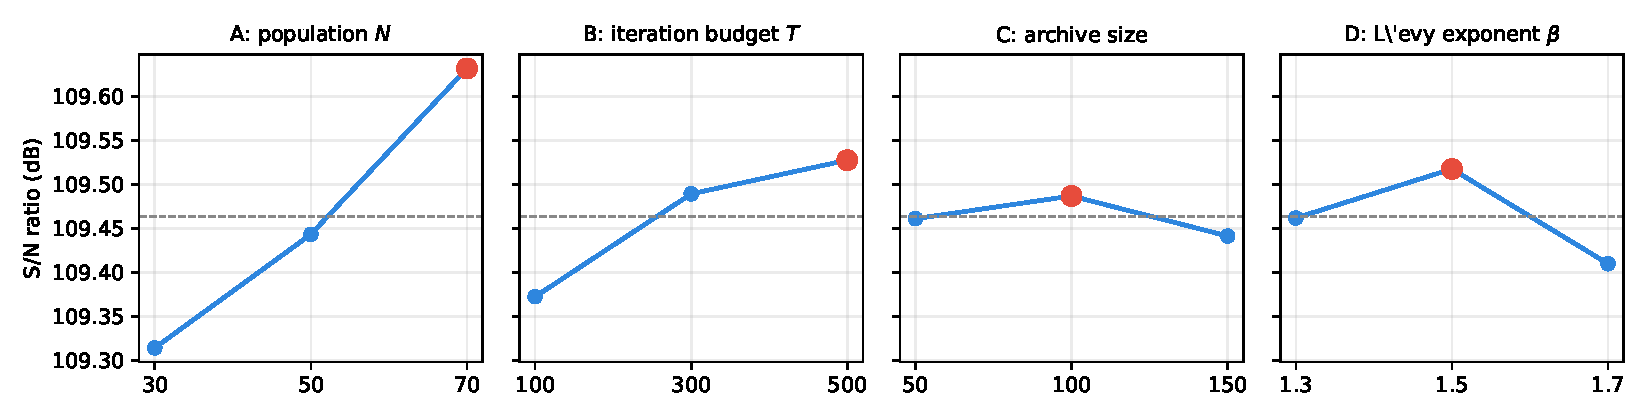
\includegraphics[width=\textwidth]{taguchi_main_effects.pdf}
\caption{Main-effects plot of the S/N ratio. The dashed line is the grand mean (109.46~dB) and the red star the best level per factor; population and iteration budget show clear trends (population the steeper), while archive size and $\beta$ are essentially flat.}
\label{fig:taguchi}
\end{figure}


%===============================================================================
\section{Results}
\label{sec:results}

\subsection{Combined Pareto front and domination of FIFO}
\label{sec:front}

Combining and re-filtering the 30 runs yields a front of 104 non-dominated solutions; the FIFO baseline lies strictly inside the dominated region. The extreme solutions expose the trade-offs: the minimum-$f_2$ solution reaches radical equity ($f_1=8.9994$, $f_2=2.0$~yr, $f_3=0$), the minimum-$f_3$ solution attains full utilization ($8.996$, $2.46$, $0$), and the minimum-$f_1$ solution is the one that dominates FIFO (below).

The central empirical finding is that FIFO is not Pareto-optimal: the minimum-$f_1$ solution Pareto-dominates it---strictly better on waste ($f_3$ from 1{,}940 to 680 visas), tied on the maximal disparity ($f_2=13.0$), and only negligibly better on the near-degenerate $f_1$ (8.7891 to 8.7884). The substantive case against FIFO is thus about waste and equity: 94 of the 104 front solutions reach $f_3=0$ (zero waste, which FIFO never attains), with disparities spanning from 13.0 years down to 2.0. (The MOHHO, Discrete-MOHHO, and perm-NSGA-II combined fronts agree within $0.3\,\%$ in hypervolume.)

\paragraph{Convergence and robustness.}
The mean hypervolume reaches 95\,\% of its final value by iteration~5 and 99\,\% by iteration~135. Over the 30 runs the \HV\ distribution is narrow (mean $302{,}756$, coefficient of variation [CV] $2.36\,\%$), evidencing a stable, reproducible algorithm.

\subsection{Decoder, representation, and search: a controlled ladder}
\label{sec:ablation}

We attribute performance to its true source by climbing a ladder of methods, all sharing the decoder and a $25{,}000$ function-evaluation budget (Table~\ref{tab:ladder}, Figure~\ref{fig:ladder}). The permutation-native methods inherit the Taguchi-tuned $N$ and $T$ and are not separately tuned, so any edge is not a tuning artifact. Under this budget MOHHO beats the real-coded NSGA-II by $3.2\,\%$ in mean hypervolume (paired two-sided Wilcoxon $p=4.4\times10^{-6}$, $A_{12}=0.85$) and shows lower spacing (NSGA-II edges it on \IGD\ to the combined reference front).

\paragraph{Blind sampling beats near-identity search---but not a competent swarm.}
\emph{Random restart}---blind sampling with no search---already reaches a mean \HV\ of $310{,}214$: $5.7\,\%$ above the real-coded NSGA-II and $2.5\,\%$ above the classic real-coded MOHHO (the naive swarm wins on only $10/30$ paired seeds). The decoder shapes a landscape on which blind sampling outperforms both of these real-coded searches; giving NSGA-II the identical archive barely helps it ($293{,}666$ vs.\ $293{,}367$), so its deficit is not an archiving artifact.

Nor is blind sampling's strength order-level greediness: a GRASP-style semi-greedy control~\cite{feo} ($\alpha\sim U(0,1)$, same budget and archive) lands $3.8\,\%$ below uniform constructions ($298{,}531$, $p=1.9\times10^{-9}$)---the decoder's heuristic bias~\cite{raidl} helps every construction. Nor is it tuning: NSGA-II's own L9 (nine configurations, best confirmed on the 30-seed block: $\eta_c{=}2$, $p_m{=}5/d$) climbs to $308{,}082$---a statistical tie with blind sampling ($p=0.25$), still $3.2\,\%$ below the permutation tier. A Pareto local search (single swaps are near-identity, so the diagnostic predicts failure) lands $2.0\,\%$ below blind sampling ($p=3.4\times10^{-4}$). With the registered sweep below, five controls tell one story: nothing we tested short of order renewal beats blind sampling here. To show that what fails here is degenerate search rather than real-coded search as such, we built a \emph{competent} real-coded MO-HHO: HHO movement with elitist non-dominated-sorting selection and polynomial mutation in place of the dominance-gated acceptance. It is sound where the naive swarm collapses (ZDT2 hypervolume $0.99$ vs.\ $0.20$ of the true front), and at the same $25{,}000$-evaluation budget on the visa it beats random restart ($316{,}347$ vs.\ $310{,}214$, $+2.0\,\%$, paired Wilcoxon $p=5.7\times10^{-4}$, 30 seeds).

\paragraph{Why near-identity operators fail.}
We measured why the real-coded NSGA-II falls below blind sampling. On the SPV random keys, SBX and polynomial mutation are near-identity on the decoded permutation: over $3{,}000$ trials the Kendall rank correlation between a parent's SPV order and its child's is $\tau=0.99$ (and stays in $[0.987,0.992]$ when measured on-trajectory). Sweeping the crossover distribution index $\eta_c\in\{2,\dots,100\}$ confirms this is no tuning artifact: even the most disruptive setting ($\eta_c{=}2$, $\tau{=}0.92$) leaves the GA's mean \HV\ at $305{,}293$, below blind random restart. The GA perturbs the keys so little that the induced permutation barely changes, leaving it almost frozen in combinatorial space. HHO's position updates, by contrast, propose large permutation jumps ($\tau\approx0$) that the dominance-gated acceptance rarely admits (only ${\sim}0.6\,\%$ of hawks move per iteration), but the archive keeps the rejected proposals---hence MOHHO $>$ NSGA-II within the random-key tier. The real-coded MOHHO is thus a deliberately standard, weak baseline (its ZDT2 collapse persists under every acceptance rule and repair we tried): our thesis rests on degenerate real-coded search losing even to blind sampling, not on the swarm being strong.

\paragraph{Matching the operators to the representation.}
The clean fix is to act directly on permutations. Doing so lifts four distinct paradigms above blind sampling: permutation-NSGA-II (dominance/GA) reaches $318{,}151$, permutation-SPEA2 (strength-Pareto) $317{,}135$, Discrete-MOHHO (swarm) $316{,}792$, and permutation-MOEA/D (decomposition) $314{,}846$---and the competent random-key swarm joins them ($316{,}347$), so the encoding is not the divider. The four cluster within about $1\,\%$ of one another (permutation-SPEA2 vs.\ permutation-NSGA-II: $p=0.47$, a statistical tie), yet all sit $1.5$--$2.6\,\%$ above blind random restart. Discrete-MOHHO improves on classic MOHHO by $+4.6\,\%$ (paired Wilcoxon $p=9.3\times10^{-10}$, better on all $30/30$ seeds); the most stable methods are matched ones (permutation-NSGA-II CV $0.58\,\%$, Discrete-MOHHO $0.71\,\%$, vs.\ classic MOHHO $2.36\,\%$), permutation-NSGA-II leading Discrete-MOHHO by $+0.43\,\%$ in mean \HV. Discrete-MOHHO is a mechanism check rather than the champion: made representation-matched, the swarm reclaims the top tier and low variance (replacing Discrete-MOHHO's energy schedule by run-average constants shifts \HV\ by $+0.01\,\%$, $p=0.87$---the metaphor's scheduling is not a measurable driver here~\cite{aranha,sorensen}).

\paragraph{The two conditions, graded by a predictive test.}
The ladder suggests a two-condition rule for this landscape: a method beats blind sampling only if its operator changes the decoded order ($\tau$ far from $1$) and its selection preserves population diversity (non-dominated sorting, strength-Pareto, decomposition, or a crowded archive---not dominance-gated acceptance). NSGA-II fails the first; the naive MOHHO fails the second; the competent MO-HHO and all four permutation-native methods satisfy both and beat random restart. We then tested the rule predictively on a method not used to formulate it: the rk-NSGA-II (biased uniform) of Section~\ref{sec:nsga}, whose BRKGA-style crossover changes the decoded order ($\tau=0.63\pm0.07$) under unchanged diversity-preserving selection. Read as a binary conjunction, the rule predicts a win over blind sampling. It does not: its mean \HV\ of $309{,}970$ is a statistical tie with random restart ($310{,}214$; paired Wilcoxon $p=0.79$, $A_{12}=0.47$), far above the SBX baseline ($+5.7\,\%$) yet $2.6\,\%$ below the permutation tier; a canonical BRKGA ($20\,\%$ elites, $15\,\%$ mutants, same crossover) lands at the same level ($309{,}928$). The test refines the rule rather than confirming its strongest form: both conditions are necessary but not sufficient. Holding the diversity-preserving selection fixed while varying only the operator gives an ordered four-point sequence---$\tau{=}0.99\!\to\!293{,}367$; $\tau{=}0.92\!\to\!305{,}293$; $\tau{=}0.63\!\to\!309{,}970$; $\tau{\approx}0\!\to\!315{,}730$ (Section~\ref{sec:twoconditions})---in which only near-complete order renewal clears blind sampling. A second registered sweep shows this is a family contrast, not a dose--response (predictions committed before running: the biased-uniform crossover's inheritance probability $\rho_e$, eleven levels spanning $\tau\in[0.42,1.0]$, fixed selection, all five structures, 30 seeds per level). Within the family, hypervolume is nearly flat in $\tau$ on every structure (bootstrap 95\,\% confidence intervals (CIs) bound the dose effect within ${\sim}1$ percentage point of blind sampling per $0.1\,\tau$; Spearman $-0.07$--$0.48$, n.s.), while IGD$^{+}$ against the pooled sweep front does degrade as $\tau\to1$ on three of the five ($\rho\ge0.80$). So $\tau$ is a flag, not a dial; the residual dose effect is visible only to a coverage metric. The diagnostic therefore reads: failing either condition predicts falling to or below blind sampling where it is strong; beating it requires the right kind of order renewal.

\paragraph{An empirical regularity.}
The ladder (Figure~\ref{fig:ladder}) makes the pattern unmistakable: performance is governed by whether the search is \emph{non-degenerate}---operators that change the decoded order together with selection that preserves diversity---not by the encoding (random-key versus permutation) or the metaheuristic family. That encoding--operator mismatch can hurt search has been known since random keys were introduced~\cite{bean}, with the locality of decoder-based encodings formalized by Rothlauf~\cite{rothlauf} and measured by Raidl and Gottlieb~\cite{raidl}; our contribution is the controlled, multi-method, causally graded demonstration on a real constrained multi-objective problem---including that both real-coded searches fall below blind sampling. That four distinct paradigms (swarm, decomposition, strength-Pareto, dominance/GA) converge to within about $1\,\%$ once the representation is matched is strong evidence that the family is second-order here. The two conditions (order-changing operators and diversity-preserving selection) are first-order: necessary, and graded in the operator's order disruption (the predictive test above); a competent random-key swarm satisfies both and joins the top tier, so the encoding itself is not the divider. Within a matched representation both the operator set and the selection architecture are second-order---a $3\times3$ operator${}\times{}$architecture factorial (OX${+}$swap, PMX (partially-mapped crossover)${+}$insertion, CX (cycle crossover)${+}$inversion $\times$ three of the architectures: perm-NSGA-II, perm-MOEA/D, and Discrete-MOHHO; 30 seeds) attributes only $5.5\,\%$ and $13.4\,\%$ of the hypervolume variance to them, against $78\,\%$ seed noise. A paired Friedman test with a Nemenyi post-hoc~\cite{demsar} across all nine ladder methods rejects equal performance decisively ($\chi^2=133.8$, $p\approx4.6\times10^{-25}$, critical difference $2.19$). The mean ranks order the methods as the two-condition account predicts (permutation-NSGA-II $2.97$ best, real-coded NSGA-II $8.77$ worst; rk-NSGA-II $4.57$, within the critical difference of random restart $6.47$); finer within-tier gaps fall inside the critical difference. All twelve headline pairwise claims survive a Holm correction over the named family. Re-scoring every per-run front under IGD$^{+}$ and additive $\epsilon$ against a common nine-method reference front preserves the structure (rank correlations $0.82$/$0.85$ with the \HV\ ranking; the four both-condition methods hold the top four ranks under all three indicators, permutation-SPEA2 best under both reference-free ones; permutation-MOEA/D is the one displacement). We frame this as an empirical regularity for this problem, not a general law; the structurally distinct problems of Section~\ref{sec:secondproblem} address generality.

\begin{table}[t]
\centering
\caption{The method ladder: 30 runs each, identical greedy decoder and $25{,}000$-evaluation budget. Top block: random-key encoding (including the BRKGA-style predictive-test method and a competent MO-HHO that reaches the top tier); bottom block: permutation-native. A competent random-key method matches the permutation tier, so the encoding is not the performance divider---non-degenerate search is. Best per column in bold (rk-NSGA-II's combined front benefits from its high between-run dispersion---its bimodal runs explore different regions---while per-run it only ties blind sampling); ``perm-'' abbreviates ``permutation-''.}
\label{tab:ladder}
\small
\begin{tabular}{llccrr}
\toprule
\textbf{Method} & \textbf{Paradigm} & \textbf{Mean \HV\ $\pm\,\sigma$} & \textbf{CV} & \textbf{Comb.\ \HV} & \textbf{\#\,sols}\\
\midrule
NSGA-II            & GA       & $293{,}367 \pm 6{,}996$ & 2.38\,\% & 316{,}060 & 92\\
MOHHO              & swarm    & $302{,}756 \pm 7{,}138$ & 2.36\,\% & 320{,}984 & 104\\
rk-NSGA-II (biased unif.) & GA & $309{,}970 \pm 9{,}790$ & 3.16\,\% & \textbf{325{,}465} & 157\\
Random restart     & ---      & $310{,}214 \pm 2{,}735$ & 0.88\,\% & 317{,}673 & 65\\
Competent MO-HHO   & swarm    & $316{,}347 \pm 6{,}683$ & 2.11\,\% & 321{,}800 & \textbf{207}\\
\midrule
perm-MOEA/D                 & decomp.\ & $314{,}846 \pm 5{,}384$  & 1.71\,\% & 320{,}969 & 90\\
Discrete-MOHHO              & swarm    & $316{,}792 \pm 2{,}258$  & 0.71\,\% & 321{,}408 & 137\\
perm-SPEA2                  & str.-Pareto & $317{,}135 \pm 3{,}814$ & 1.20\,\% & 322{,}037 & 179\\
perm-NSGA-II                & GA       & $\mathbf{318{,}151 \pm 1{,}855}$ & \textbf{0.58\,\%} & 321{,}935 & 148\\
\bottomrule
\end{tabular}
\end{table}

\begin{figure}[t]
\centering

\includegraphics[width=0.74\textwidth]{ladder.pdf}
\caption{The nine-method ladder: per-run hypervolume (30 runs each, identical decoder and budget). The divider is non-degenerate search, not the encoding: within the random-key block (left, shaded amber) the BRKGA-style rk-NSGA-II rises to---but only ties---blind random restart, while the competent MO-HHO joins the permutation-native top tier (right, shaded blue).}
\label{fig:ladder}
\end{figure}

\paragraph{Robustness to a search-space-collapse confound.}
Does the decoder's budget saturation make the optimizer necessarily second-order? We tested this on three axes. \emph{Structure}: $50{,}000$ random permutations decode to $39{,}401$ distinct objective points (degeneration ratio $1.27$), and a principal-component analysis places about $99\,\%$ of the front's variance in two components (the first alone captures only $0.81$--$0.91$): a near-mono-objective instance with one wide axis ($f_2$) and a genuine but narrow second axis. \emph{Decoder}: re-running the full ladder on two \emph{non-saturating} decoders (fractional-intensity and stochastic-skip, both feasible by construction) keeps the permutation tier significantly above the random-key tier under all three decoders (paired Wilcoxon $p<10^{-3}$) and never inverts it; the margin shrinks from $6.9\,\%$ (greedy) to $4.3\,\%$ (stochastic-skip) and $1.4\,\%$ (fractional-intensity), so saturation amplifies---it does not create---the effect, and an exact $(f_1,f_3)$ MILP front ($f_2$---differences of ratios of decision variables---is outside MILP form and evaluated a posteriori) exposes no practically meaningful non-saturating solution the greedy front misses. \emph{Metric}: the per-run tier ranking is reference-point-robust (the strict split holds under four of five reference points), though on combined fronts the strict tier softens under reference-free metrics (\IGD$^{+}$, additive $\epsilon$), and the hypervolume exhibiting it is dominated by the wide $f_2$ axis. The confound thus bounds rather than overturns the claim: the effect is real and robust, modest on this saturation-amplified, $f_2$-dominated instance, with the general regularity resting on the additional structures below.

\subsection{Isolating the two conditions: a controlled $2\times2$}
\label{sec:twoconditions}
The ladder establishes the two conditions by observation; we now isolate each condition with a controlled $2\times2$ on a single real-coded random-key skeleton---same greedy decoder, instance, $25{,}000$-evaluation budget, and 30 seeds---varying only the \emph{operator} (order-changing HHO moves with mutation, $\tau\!\approx\!0$, versus near-identity SBX, $\tau\!=\!0.99$) and the \emph{selection} (diversity-preserving non-dominated sorting (NDS) versus dominance-gated acceptance). Table~\ref{tab:factorial2x2} shows that only the cell satisfying both conditions beats blind random restart ($315{,}730$ versus $310{,}214$~\HV, $+1.78\,\%$, paired Wilcoxon $p=1.4\times10^{-3}$, $A_{12}=0.79$); either single-condition cell falls below blind sampling. Gated acceptance freezes the population (only $0.9\,\%$ of individuals move per iteration), and near-identity SBX leaves the decoded order almost unchanged even when the population does move. Crucially, the two conditions are synergistic, not additive: a two-factor analysis of variance finds a significant operator$\times$selection interaction ($\eta^2=0.098$, $F=16.7$, $p=8.0\times10^{-5}$; a permutation test agrees, $p=2.0\times10^{-4}$), alongside main effects of $\eta^2=0.076$ (operator) and $\eta^2=0.145$ (selection). Each effect is modest against seed noise; the interaction matters because it separates beating blind sampling from losing to it. Neither condition alone lifts performance above blind sampling (both single-condition cells lose by $1.4$--$2.0\,\%$). Figure~\ref{fig:mech2x2} maps each cell onto its operator $\tau$ and realized population movement, isolating the winning cell in the low-$\tau$, high-movement corner. 

\begin{table}[t]
\centering
\caption{Controlled $2\times2$ isolating the two conditions on one real-coded random-key skeleton (visa decoder, 30 seeds, $25{,}000$ evaluations). Only the cell that both changes the decoded order and preserves diversity beats blind random restart ($310{,}214$~\HV); the operator$\times$selection interaction is significant. Best in bold.}
\label{tab:factorial2x2}
\small
\begin{tabular}{llrrr}
\toprule
\textbf{Operator} & \textbf{Selection} & \textbf{Mean \HV} & \textbf{vs.\ random} & \textbf{$A_{12}$}\\
\midrule
order-changing ($\tau\!\approx\!0$) & diversity (NDS) & $\mathbf{315{,}730}$ & $\mathbf{+1.78\,\%}$ & $\mathbf{0.79}$\\
order-changing ($\tau\!\approx\!0$) & gated            & $304{,}126$ & $-1.96\,\%$ & $0.24$\\
near-identity ($\tau\!=\!0.99$)     & diversity (NDS) & $305{,}892$ & $-1.39\,\%$ & $0.34$\\
near-identity ($\tau\!=\!0.99$)     & gated            & $304{,}760$ & $-1.76\,\%$ & $0.21$\\
\bottomrule
\end{tabular}
\end{table}

\begin{figure}[t]
\centering
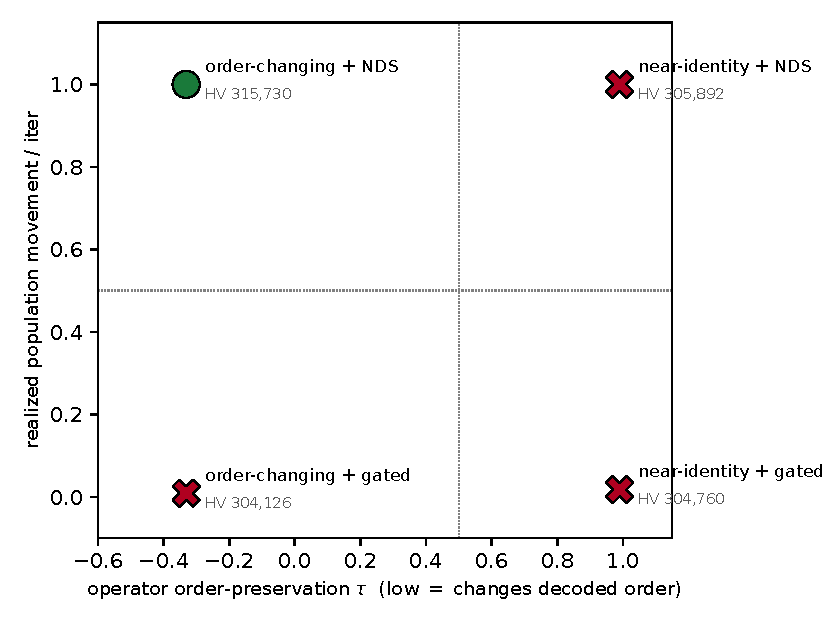
\includegraphics[width=0.65\textwidth]{mechanism_2x2.pdf}
\caption{Mechanism of the two conditions across the $2\times2$ cells: operator order-preservation $\tau$ versus realized population movement per iteration, with each cell's mean \HV. Only the cell meeting both conditions occupies the favorable low-$\tau$, high-movement corner and beats blind sampling.}
\label{fig:mech2x2}
\end{figure}

\subsection{Generalization across instances}
\label{sec:generalization}

To check robustness to the demand estimate, we built five further instances perturbing every group's demand by an independent uniform $\pm 20\,\%$ (fixed seeds) and recomputing the spillover-adjusted category and per-country caps. On all five---as on the base instance---FIFO is dominated, MOHHO's mean \HV\ exceeds NSGA-II's (one-sided Mann--Whitney with 10 seeds, $p\le0.071$ per instance: directionally consistent on five of five, two individually significant; as perturbations of one instance, this is descriptive robustness, not confirmatory evidence), and random restart matches or exceeds MOHHO ($101$--$103\,\%$ of its \HV) while both stay above NSGA-II ($96$--$99\,\%$ of MOHHO). 

\subsection{Generalization across structurally distinct problems}
\label{sec:secondproblem}

We replicate the six-method core of the ladder on three further classic structures sharing nothing with visa allocation but the SPV${}+{}$greedy/permutation methodology: a 0/1 multidimensional knapsack (MOMKP, a \emph{selection} landscape), a tri-objective traveling salesman (mo-TSP, \emph{sequencing}), and a tri-objective permutation flow-shop (mo-PFSP, \emph{scheduling}); same budget, 30 common seeds, paired Friedman${}+{}$Nemenyi (Table~\ref{tab:structures}). One result is robust across all four structures: among the six core ladder methods the best optimizer is always a permutation-native method, and neither blind random restart nor any naive real-coded method ever wins---with the family second-order among matched methods (all four omnibus tests reject equality, $\chi^2=112$--$150$, $p<10^{-21}$). We further placed the competent random-key MO-HHO of Section~\ref{sec:ablation} on all four structures (seven methods, same 30-seed budget): it wins outright on the knapsack (mean rank 1.13 of seven, above every permutation-native method) and ranks 2nd, 2nd, and 5th on the visa, flow-shop, and TSP, where a permutation-native method remains the single best. So the cross-structure regularity is sharper than ``permutation beats random-key'': what wins among the ladder methods on every structure is one satisfying both conditions---permutation-native on three of the four, the competent random-key swarm on the knapsack. Discrete-MOHHO is top-two on three of the four and the most stable matched method. What does not generalize is the dramatic ``GA below random sampling'': it holds on the selection landscapes (visa, knapsack, where the real-coded NSGA-II is worst) but reverses on the sequencing landscapes (TSP, flow-shop, where it is competitive and random restart is worst instead). The mechanism: operator order-preservation is problem-independent ($\tau\approx0.99$), but its consequence is landscape-dependent---near-identity SBX freezes search on selection landscapes yet acts as useful local search on sequencing ones. Tuning sharpens this: NSGA-II's own L9 on the knapsack lifts it $46\,\%$ above blind sampling ($p=1.9\times10^{-9}$; again via $p_m{=}5/d$)---the knapsack collapse is a default-configuration artifact; the configuration-robust collapse is the visa's alone. A fifteen-point capacity sweep rules out a single headroom scalar (it moves opposite to the hypothesis; Spearman $\rho=-0.78$, $p=0.001$, descriptive). The transferable regularity is thus precise: the best ladder method on every structure satisfies both conditions; the GA-collapse is landscape-specific.

\paragraph{A registered prospective test.}
As a final check we registered the diagnostic's four predictions for a fifth, unseen problem before running any optimizer on it (the registration commit precedes the results in the repository): a tri-objective set-covering problem (mo-SCP; 150 elements, 120 sets, three cost vectors; the SPV decoder adds a set iff it covers a new element), labeled a selection landscape by its subset structure. The two predictions following from the two conditions alone held: permutation-NSGA-II and the competent swarm beat blind sampling decisively ($p=9.3\times10^{-10}$, $A_{12}=1.0$ for both). The two tied to the landscape label failed, informatively: the real-coded NSGA-II finishes $10\,\%$ above blind sampling and the biased-uniform rk-NSGA-II is the single best method ($+60\,\%$, above even permutation-NSGA-II). Mechanistically, mo-SCP saturates no shared budget---every decode is a feasible cover and marginal reorderings swap one set---so it behaves like a sequencing landscape (local search useful, blind sampling weak). The test confirms the two-condition core (the best ladder method on all five structures satisfies both conditions) and falsifies the surface label as a classifier (the confirmed half carried less falsification risk on this blind-sampling-weak landscape). The operative determinant remains the registered open question; we hypothesize decoder budget saturation, consistent with the headroom anti-correlation. A first operationalization---the saturation share $s$ over random decodes, seconds to compute---retrodicts the default-collapse split ($s\approx1$ visa/knapsack, $0$ elsewhere) but awaits a registered test on unseen problems.

\begin{table}[t]
\centering
\caption{Mean Friedman rank (lower is better; 30 paired seeds) on four structurally distinct problems. A permutation-native method (pm) is best on every structure among the six core methods (\textbf{bold}); at its default configuration the real-coded NSGA-II falls below random restart only on the selection landscapes (visa, knapsack; tuning rescues the knapsack---see text). ``rk'' $=$ random-key.}
\label{tab:structures}
\small
\begin{tabular}{llcccc}
\toprule
\textbf{Method} & \textbf{Enc.} & \textbf{Visa} & \textbf{Knapsack} & \textbf{TSP} & \textbf{Flow-shop}\\
\midrule
perm-NSGA-II        & pm & \textbf{1.60} & \textbf{1.10} & 2.00 & \textbf{1.80}\\
perm-MOEA/D         & pm & 2.53 & 2.87 & \textbf{1.00} & 2.83\\
Discrete-MOHHO      & pm & 2.23 & 2.10 & 4.00 & 2.63\\
\midrule
MOHHO (real-coded)  & rk & 4.67 & 3.93 & 5.00 & 5.07\\
Random restart      & rk & 4.20 & 5.23 & 6.00 & 5.93\\
NSGA-II (real-coded)& rk & 5.77 & 5.77 & 3.00 & 2.73\\
\bottomrule
\end{tabular}
\end{table}

%===============================================================================
\section{Discussion}
\label{sec:discussion}

\paragraph{The trade-off is structural.}
Two countries hold roughly three-quarters of demand with 10--13-year waits; the $7\,\%$ ceiling forbids fully serving them, so reducing disparity ($f_2$) leaves unserved load ($f_1\!\uparrow$) and equitable spreading idles saturated categories ($f_3\!\uparrow$). The three extreme solutions (Section~\ref{sec:front}) are mutually non-dominated---genuine three-way conflict. We keep $f_1$ distinct (its range is an order of magnitude narrower than $f_2$'s) because the minimum-$f_1$ policy is the one that dominates FIFO.

\paragraph{A diagnostic protocol, and policy.}
The ladder distills into a cheap a priori protocol: (1)~draw ${\sim}3{,}000$ parent--child pairs through the candidate operators and measure the Kendall $\tau$ of the decoded orders; (2)~check that selection preserves diversity (NDS, strength-Pareto, decomposition, or a crowded archive---not gated acceptance); (3)~measure how strong blind sampling is on the decoded space (run it; it is the cheapest method) rather than classifying by surface structure---our registered prospective test (Section~\ref{sec:secondproblem}) shows the label can mispredict. The prospectively validated core: the best ladder method on all five structures satisfies both conditions, and order-renewal methods beat blind sampling on all five. On the budget-saturating problems, failing either check predicted default-configuration performance at or below blind sampling (the one nominal exception---the naive knapsack swarm---lies within the critical difference); on the visa, where blind sampling sits within $2.6\,\%$ of the best tier, no random-key GA configuration beats it. Where blind sampling is weak, other routes to order disruption suffice: local search on sequencing problems, or a higher mutation rate (the knapsack's tuned GA). The registered sweep shows $\tau$ is a flag, not a dial. The protocol complements general fitness-landscape analysis~\cite{malan}: it measures the operator--decoder interaction rather than the landscape alone. Invest in the decoder and representation before the search heuristic; for a dependable single run, permutation-NSGA-II is strongest here. For policy, the front is a quantified menu under the assumed model: cutting disparity from 13.0 to 2.0 years costs only $\sim$$2.4\,\%$ in $f_1$ relative to FIFO---consistent with per-country-cap reform proposals~\cite{crs,fwd}; each solution maps to an auditable per-country reallocation.

\paragraph{Limitations.}
The model covers a single fiscal year, uses 21 representative countries, aggregates each group to a single priority date (within-group distributions are not modeled), and assumes every assigned visa is used. On the data: the country-level totals are anchored to published aggregates~\cite{cato,uscis,dos}, but the per-(country, category) split and priority dates are a plausible synthetic disaggregation (only India, China, the Philippines, and Mexico have category-level demand grounded in published data). These affect external validity, not the internal comparison: the ladder methods share identical data, decoder, and budget. \emph{Ethically}, $f_2$ encodes one contestable notion of fairness and treats nationalities as allocation buckets; we therefore present the front as auditable decision support, never an autonomous decision-maker, and the per-country figures illustrate method behavior rather than recommend real allocations. A post-hoc audit with alternative country-wait metrics (wait standard deviation $3.14\to0.75$, Gini $0.79\to0.17$, Jain $0.80\to0.94$) supports the same equity reading.

%===============================================================================
\section{Conclusions}
\label{sec:conclusions}

We formulated a calibrated instance of the annual allocation of U.S.\ employment-based visas as a three-objective integer program with six hard constraints and searched the decoder-reachable trade-off space through a feasibility-preserving SPV${}+{}$greedy decoder that guarantees feasibility by construction---no penalties, no repair. A Taguchi L9 design fixed a common, confirmed operating point for every method. Across 30 independent runs the recovered Pareto front dominates the FIFO incumbent---chiefly by reducing waste while essentially matching its waiting load and maximal disparity---with 94 zero-waste solutions.

Our central result comes from a controlled nine-method ladder: blind random sampling beats a standard real-coded NSGA-II and the naive real-coded MOHHO swarm, but a competent real-coded swarm (HHO with non-dominated-sorting selection) beats blind sampling by $2.0\,\%$---so what fails is degenerate search, not real-coded search as such. The lesson is a two-condition diagnostic, scoped and graded. At default configuration on the budget-saturating problems---and under every configuration on the visa---a method that does not change the decoded order or does not preserve population diversity falls to or below blind sampling (within the critical difference). In a predictive test, a method not used to formulate the rule---a BRKGA-style biased-uniform crossover that does change the order ($\tau=0.63$) under diversity-preserving selection---only ties blind sampling, so the two conditions are necessary but not sufficient. A second registered sweep (one operator, a continuous disruption knob, eleven levels, all five structures) finds hypervolume nearly flat in $\tau$ within the family: the four-point gradient was a family contrast, not a dose--response, and only the right kind of order renewal ($\tau\approx0$ moves or permutation operators) reaches the visa top tier. There, four permutation-native paradigms and a competent random-key swarm cluster within about $1\,\%$---so the divider is non-degenerate search, not the encoding; Discrete-MOHHO improves on classic MOHHO by $4.6\,\%$ and is the most stable swarm, within $0.5\,\%$ of permutation-NSGA-II.

The FIFO-domination and decoder-dominance findings are directionally consistent across five perturbed-demand instances, and a four-structure study (the visa plus knapsack, TSP, flow-shop) sharpens what generalizes: the best ladder method on every structure satisfies both conditions (permutation-native on three, the competent random-key swarm on the knapsack) and the family is second-order among matched methods (the robust, transferable regularity), whereas the collapse of a mismatched GA below blind sampling occurs at default configuration on the budget-saturating landscapes and is configuration-robust only on the visa, where five controls show that nothing we tested short of order renewal beats blind sampling---on TSP and flow-shop the same near-identity operators act as useful local search and the GA is competitive. A registered prospective test on a fifth problem (set covering) confirms the core (the best ladder method again satisfies both conditions) and falsifies the surface landscape label; the determinant (we hypothesize: decoder budget saturation) remains the registered open question. Order-preservation is problem-independent; whether it freezes or refines is landscape-dependent (a headroom scalar is ruled out: $\rho=-0.78$, $p=0.001$).

Beyond the numbers, the method yields an auditable menu of feasible trade-offs as decision support, not a policy prescription. Future work includes a multi-period formulation, the full country roster, and testing the registered budget-saturation hypothesis as the landscape determinant.

%===============================================================================
\subsubsection*{Data and Code Availability.}
The data, optimizer, Taguchi design, and all scripts are available at \url{https://github.com/jrebull/MIAAD_Harrisv2} (tag \texttt{micai-submission-v1}); fixed seeds (diagnostic suite: 1; comparisons: 1--30) regenerate every reported number deterministically.
% >>> REVIEW: remove the URL above for double-blind submission.

\subsubsection*{Acknowledgments.}
% >>> REVIEW: omit this block for double-blind submission.
The authors thank the Universidad Aut\'onoma de Ciudad Ju\'arez for institutional support.

%===============================================================================
\begin{thebibliography}{99}

\bibitem{alrafei}
Al Rafei, T., Yousfi Steiner, N., Chrenko, D.: Genetic algorithm and Taguchi method: an approach for better Li-ion cell model parameter identification. Batteries \textbf{9}(2), 72 (2023). \doi{10.3390/batteries9020072}

\bibitem{aranha}
Aranha, C., Camacho Villal\'on, C.L., Campelo, F., Dorigo, M., Ruiz, R., Sevaux, M., et al.: Metaphor-based metaheuristics, a call for action: the elephant in the room. Swarm Intelligence \textbf{16}(1), 1--6 (2022). \doi{10.1007/s11721-021-00202-9}

\bibitem{bansak}
Bansak, K., Ferwerda, J., Hainmueller, J., Dillon, A., Hangartner, D., Lawrence, D., et al.: Improving refugee integration through data-driven algorithmic assignment. Science \textbf{359}(6373), 325--329 (2018). \doi{10.1126/science.aao4408}

\bibitem{bean}
Bean, J.C.: Genetic algorithms and random keys for sequencing and optimization. ORSA Journal on Computing \textbf{6}(2), 154--160 (1994). \doi{10.1287/ijoc.6.2.154}

\bibitem{cato}
Bier, D.J.: 1.8 million in employment-based green card backlog. Cato Institute, Washington, DC (2023), \url{https://www.cato.org/blog/18-million-employment-based-green-card-backlog}

\bibitem{chaves}
Chaves, A.A., Resende, M.G.C., Schuetz, M.J.A., Brubaker, J.K., Katzgraber, H.G., de Arruda, E.F., et al.: A random-key optimizer for combinatorial optimization. Journal of Heuristics \textbf{31}(4), 32 (2025). \doi{10.1007/s10732-025-09568-z}

\bibitem{choo}
Choo, Y.H., Cai, Z., Le, V., Johnstone, M., Creighton, D., Lim, C.P.: Enhancing the Harris' Hawk optimiser for single- and multi-objective optimisation. Soft Computing \textbf{27}(22), 16675--16715 (2023). \doi{10.1007/s00500-023-08952-w}

\bibitem{coello}
Coello Coello, C.A., Lamont, G.B., Van Veldhuizen, D.A.: Evolutionary Algorithms for Solving Multi-Objective Problems, 2nd edn. Springer, New York (2007). \doi{10.1007/978-0-387-36797-2}

\bibitem{crs}
Congressional Research Service: U.S. employment-based immigration policy. Report R47164 (2023), \url{https://www.congress.gov/crs-product/R47164}

\bibitem{deb}
Deb, K., Pratap, A., Agarwal, S., Meyarivan, T.: A fast and elitist multiobjective genetic algorithm: NSGA-II. IEEE Transactions on Evolutionary Computation \textbf{6}(2), 182--197 (2002). \doi{10.1109/4235.996017}

\bibitem{demsar}
Demšar, J.: Statistical comparisons of classifiers over multiple data sets. Journal of Machine Learning Research \textbf{7}, 1--30 (2006), \url{https://jmlr.org/papers/v7/demsar06a.html}

\bibitem{derrac}
Derrac, J., García, S., Molina, D., Herrera, F.: A practical tutorial on the use of nonparametric statistical tests as a methodology for comparing evolutionary and swarm intelligence algorithms. Swarm and Evolutionary Computation \textbf{1}(1), 3--18 (2011). \doi{10.1016/j.swevo.2011.02.002}

\bibitem{feo}
Feo, T.A., Resende, M.G.C.: Greedy randomized adaptive search procedures. Journal of Global Optimization \textbf{6}(2), 109--133 (1995). \doi{10.1007/BF01096763}

\bibitem{fwd}
FWD.us: Per-country cap reform: priority bill spotlight (2024), \url{https://www.fwd.us/news/per-country-cap-reform-priority-bill-spotlight/}

\bibitem{garey}
Garey, M.R., Johnson, D.S.: Computers and Intractability: A Guide to the Theory of NP-Completeness. W.H. Freeman, San Francisco (1979)

\bibitem{gezici}
Gezici, H., Livatyali, H.: An improved Harris Hawks Optimization algorithm for continuous and discrete optimization problems. Engineering Applications of Artificial Intelligence \textbf{113}, 104952 (2022). \doi{10.1016/j.engappai.2022.104952}

\bibitem{goncalves}
Gon\c{c}alves, J.F., Resende, M.G.C.: Biased random-key genetic algorithms for combinatorial optimization. Journal of Heuristics \textbf{17}(5), 487--525 (2011). \doi{10.1007/s10732-010-9143-1}

\bibitem{heidari}
Heidari, A.A., Mirjalili, S., Faris, H., Aljarah, I., Mafarja, M., Chen, H.: Harris hawks optimization: algorithm and applications. Future Generation Computer Systems \textbf{97}, 849--872 (2019). \doi{10.1016/j.future.2019.02.028}

\bibitem{jangir}
Jangir, P., Heidari, A.A., Chen, H.: Elitist non-dominated sorting Harris hawks optimization: framework and developments for multi-objective problems. Expert Systems with Applications \textbf{186}, 115747 (2021). \doi{10.1016/j.eswa.2021.115747}

\bibitem{londe}
Londe, M.A., Pessoa, L.S., Andrade, C.E., Resende, M.G.C.: Biased random-key genetic algorithms: a review. European Journal of Operational Research \textbf{321}(1), 1--22 (2025). \doi{10.1016/j.ejor.2024.03.030}

\bibitem{malan}
Malan, K.M., Engelbrecht, A.P.: A survey of techniques for characterising fitness landscapes and some possible ways forward. Information Sciences \textbf{241}, 148--163 (2013). \doi{10.1016/j.ins.2013.04.015}

\bibitem{montgomery}
Montgomery, D.C.: Design and Analysis of Experiments, 9th edn. Wiley, Hoboken (2017)

\bibitem{rahimi}
Rahimi, I., Gandomi, A.H., Chen, F., Mezura-Montes, E.: A review on constraint handling techniques for population-based algorithms: from single-objective to multi-objective optimization. Archives of Computational Methods in Engineering \textbf{30}(3), 2181--2209 (2023). \doi{10.1007/s11831-022-09859-9}

\bibitem{raidl}
Raidl, G.R., Gottlieb, J.: Empirical analysis of locality, heritability and heuristic bias in evolutionary algorithms: a case study for the multidimensional knapsack problem. Evolutionary Computation \textbf{13}(4), 441--475 (2005). \doi{10.1162/106365605774666886}

\bibitem{rothlauf}
Rothlauf, F.: Representations for Genetic and Evolutionary Algorithms, 2nd edn. Springer, Berlin, Heidelberg (2006). \doi{10.1007/3-540-32444-5}

\bibitem{sorensen}
S\"orensen, K.: Metaheuristics---the metaphor exposed. International Transactions in Operational Research \textbf{22}(1), 3--18 (2015). \doi{10.1111/itor.12001}

\bibitem{tasgetiren}
Tasgetiren, M.F., Liang, Y.-C., Sevkli, M., Gencyilmaz, G.: A particle swarm optimization algorithm for makespan and total flowtime minimization in the permutation flowshop sequencing problem. European Journal of Operational Research \textbf{177}(3), 1930--1947 (2007). \doi{10.1016/j.ejor.2005.12.024}

\bibitem{uscis}
U.S. Citizenship and Immigration Services: Fiscal year 2023 employment-based adjustment of status FAQs (2023), \url{https://www.uscis.gov/green-card/green-card-processes-and-procedures/fiscal-year-2023-employment-based-adjustment-of-status-faqs}

\bibitem{dos}
U.S. Department of State: Visa bulletin for February 2026 (2026), \url{https://travel.state.gov/content/travel/en/legal/visa-law0/visa-bulletin/2026/visa-bulletin-for-february-2026.html}

\bibitem{vargha}
Vargha, A., Delaney, H.D.: A critique and improvement of the CL common language effect size statistics of McGraw and Wong. Journal of Educational and Behavioral Statistics \textbf{25}(2), 101--132 (2000). \doi{10.3102/10769986025002101}

\bibitem{cerci}
Wang, M., Wang, J.-S., Song, H.-M., Zhang, M., Zhang, X.-Y., Zheng, Y., et al.: Hybrid multi-objective Harris Hawk optimization algorithm based on elite non-dominated sorting and grid index mechanism. Advances in Engineering Software \textbf{172}, 103218 (2022). \doi{10.1016/j.advengsoft.2022.103218}

\bibitem{kusoglu}
Yüzgeç, U., Kuşoğlu, M.: Multi-objective Harris Hawks optimizer for multiobjective optimization problems. BSEU Journal of Engineering Research and Technology \textbf{1}(1), 31--41 (2020), \url{https://bseujert.bilecik.edu.tr/index.php/bseujert/article/view/14}

\bibitem{zhangli}
Zhang, Q., Li, H.: MOEA/D: a multiobjective evolutionary algorithm based on decomposition. IEEE Transactions on Evolutionary Computation \textbf{11}(6), 712--731 (2007). \doi{10.1109/TEVC.2007.892759}

\bibitem{zhang}
Zhang, W., Xiao, G., Gen, M., Geng, H., Wang, X., Deng, M., et al.: Enhancing multi-objective evolutionary algorithms with machine learning for scheduling problems: recent advances and survey. Frontiers in Industrial Engineering \textbf{2}, 1337174 (2024). \doi{10.3389/fieng.2024.1337174}

\bibitem{spea2}
Zitzler, E., Laumanns, M., Thiele, L.: SPEA2: improving the strength Pareto evolutionary algorithm. TIK-Report 103, Computer Engineering and Networks Laboratory (TIK), ETH Zurich (2001). \doi{10.3929/ethz-a-004284029}

\bibitem{zitzler}
Zitzler, E., Thiele, L.: Multiobjective evolutionary algorithms: a comparative case study and the strength Pareto approach. IEEE Transactions on Evolutionary Computation \textbf{3}(4), 257--271 (1999). \doi{10.1109/4235.797969}

\end{thebibliography}

\end{document}
